\chapter{U-Net}\label{appendix:unet}

La U-Net è stata introdotta nel $2015$ (Ronneberger et al.,~\cite{ronnebergerUNet2015}), e costituiva, allora, 
lo stato dell'arte nell'ambito della segmentazione delle immagini biomediche.

Si ribadisce che la scelta di una U-Net, nel paper di Ho et al.~\cite{ho2020}, coniuga l'esigenza che le immagini 
a monte e a valle della rete neurale abbiano le stesse dimensioni, con la peculiarità della U-Net di produrre un'immagine 
con le medesime dimensioni dell'immagine in ingresso.

In Figura~\ref{fig:UNet} è riportato il diagramma della U-Net in uno step del processo di diffusione inversa. In particolare sono mostrate esplicitamente le dimensioni
dell'immagine rumorosa $\mathbf{x}_t$ nel suo percorso attraverso la rete. Essendo un'immagine a colori, matematicamente $\mathbf{x}_t$ è un \emph{tensore}.

\begin{figure}
    \centering
    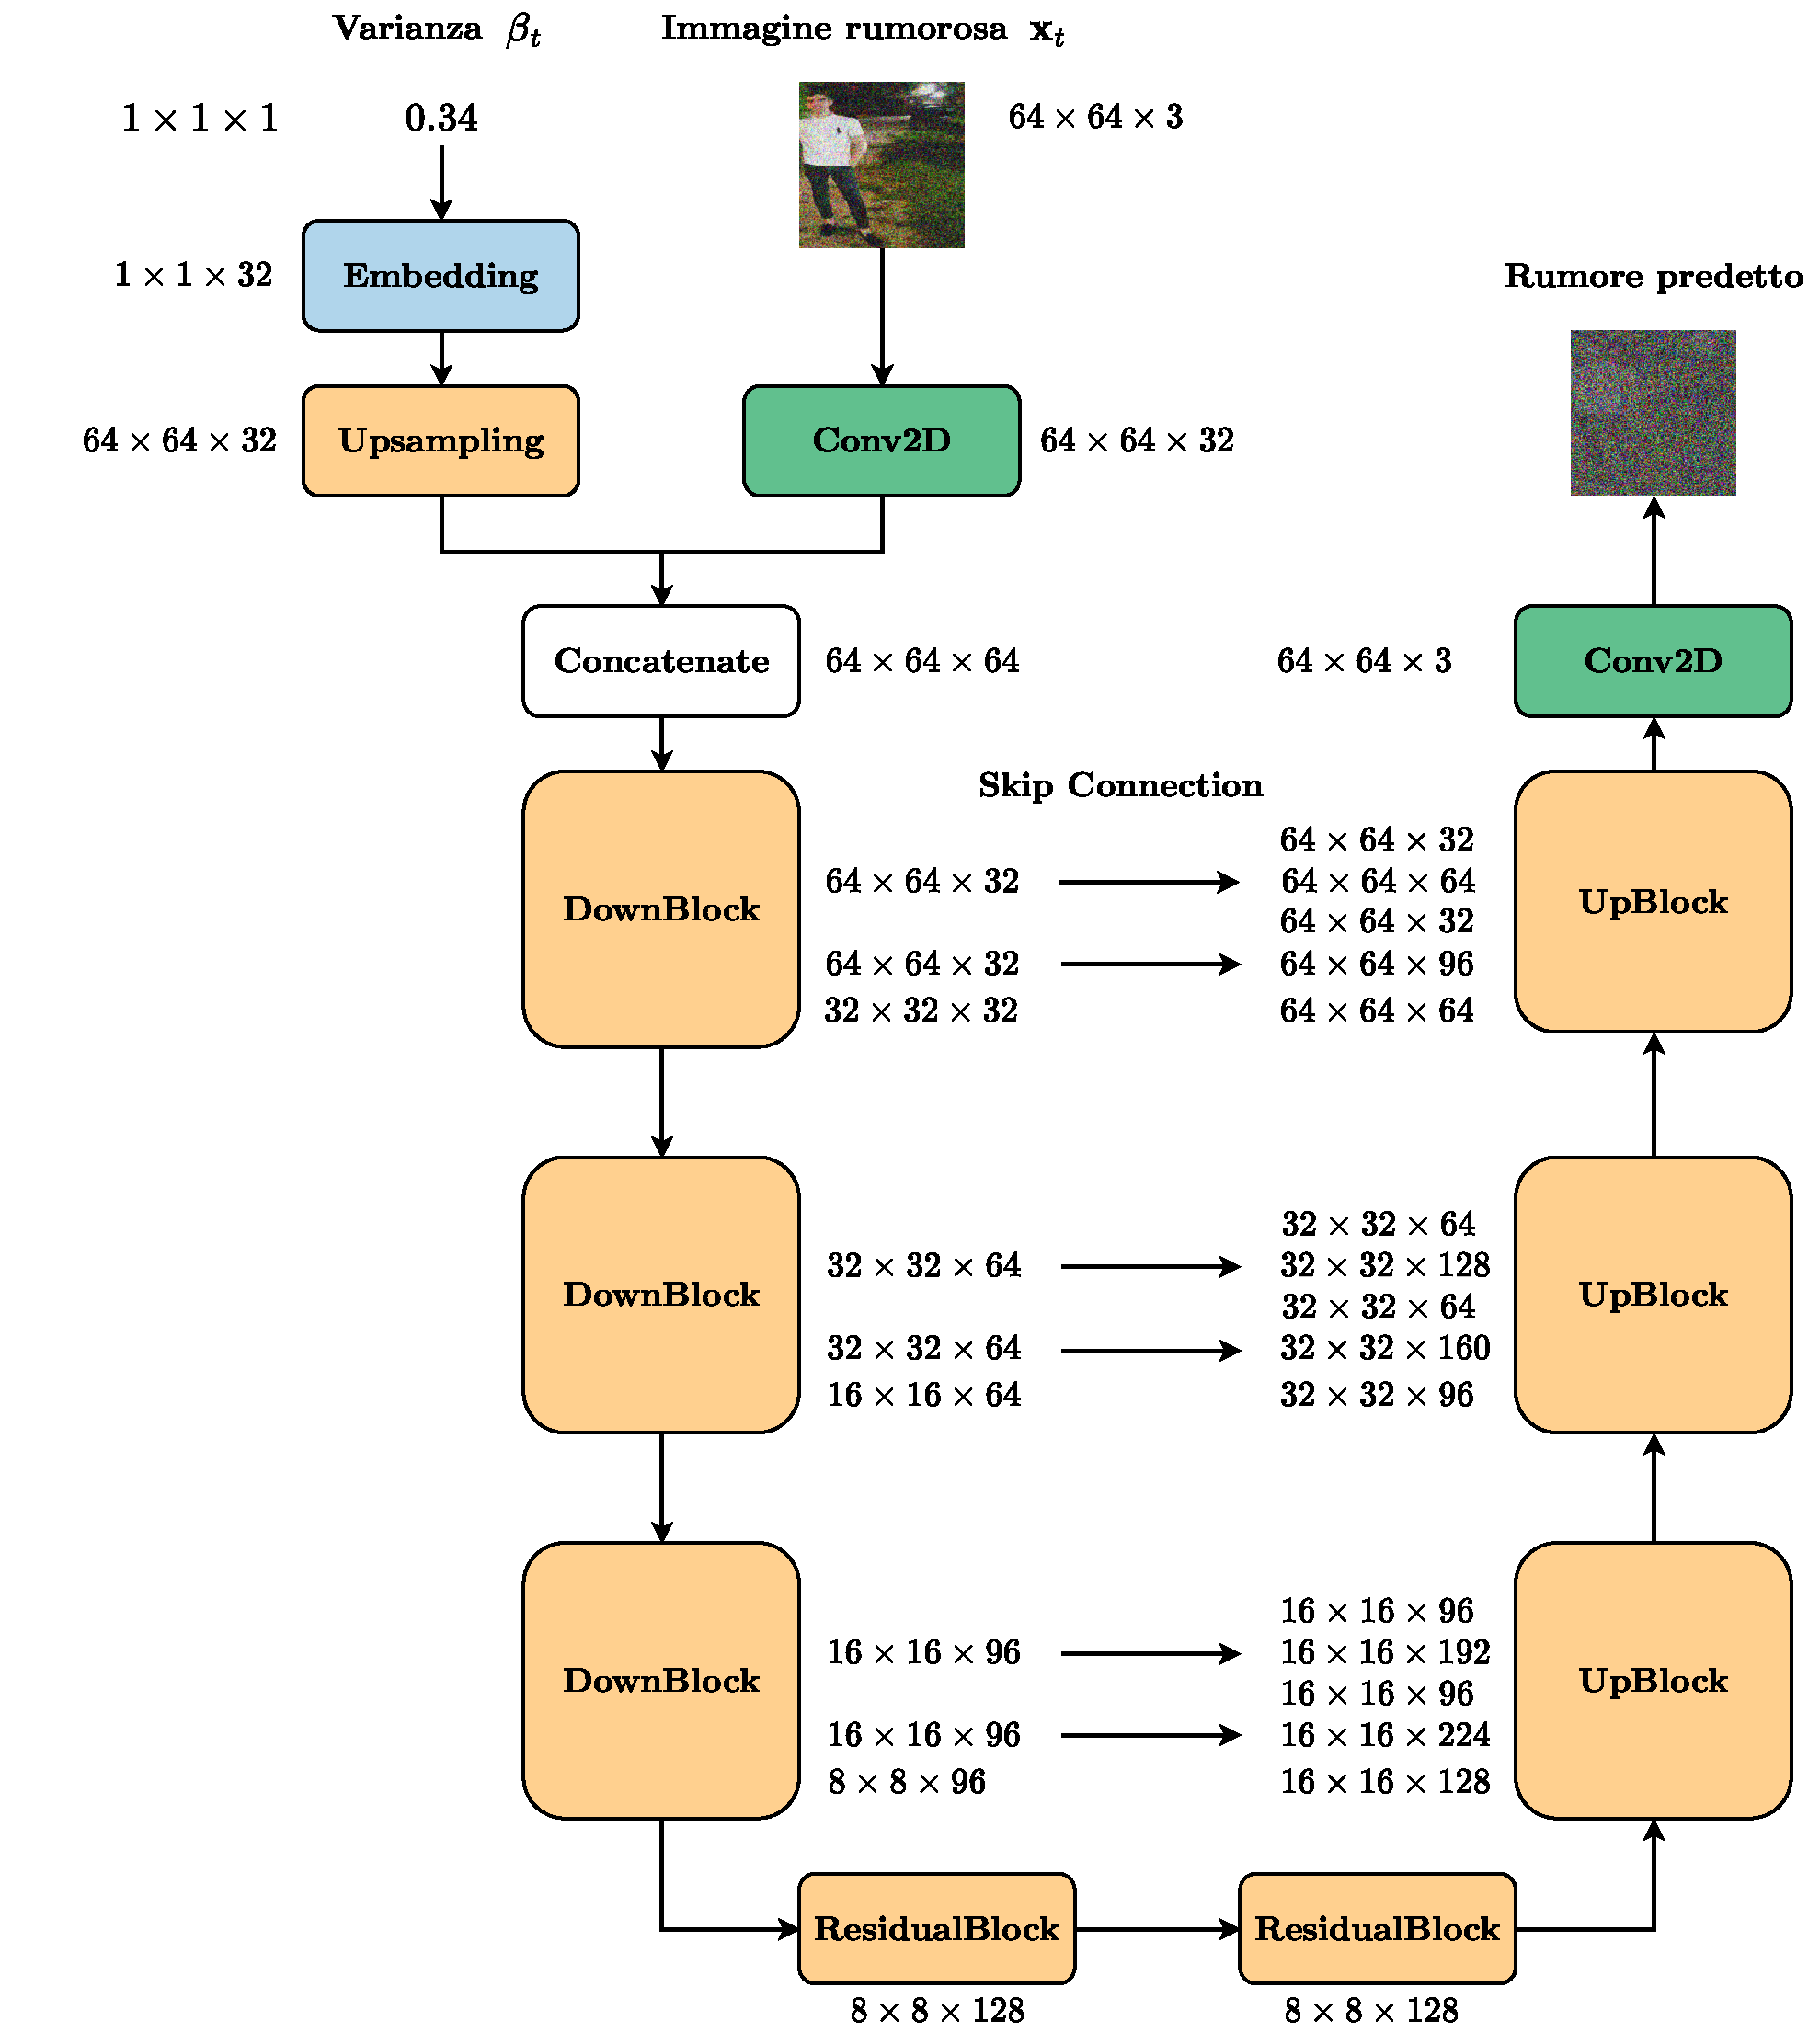
\includegraphics[keepaspectratio, scale=0.4]{UNET.pdf}
    \caption{Diagramma della U-Net in uno step della diffusione inversa. Fonte~\cite{fosterGenerativeDeepLearning2023}.}
    \label{fig:UNet}
\end{figure}

Come si evince dalla Figura~\ref{fig:UNet}, la U-Net è composta da due metà:
\begin{itemize}
\item la parte di \emph{downsampling} (a sinistra in Figura~\ref{fig:UNet}), dove l'immagine viene 
\emph{compressa spazialmente} ma \emph{espansa a livello di canale} (o profondità).
\item la parte di \emph{upsampling} (a destra in Figura~\ref{fig:UNet}), dove l'immagine viene 
\emph{espansa spazialmente} ma \emph{compressa a livello di canale}.
\end{itemize}

\noindent In Figura~\ref{fig:UNet_details} sono riportati i dettagli dei blocchi “\emph{DownBlock}” e “\emph{UpBlock}” della 
Figura~\ref{fig:UNet}. 

In particolare, relativamente all'esempio in Figura~\ref{fig:UNet}, ognuno dei blocchi “\emph{DownBlock}” nella parte di \emph{downsampling} incrementa 
il numero di canali del tensore rappresentante l'immagine mediante l'impiego di due “blocchi residuali”(\emph{ResidualBlock}), 
applicando anche un layer finale “\emph{AveragePooling2D}” per dimezzare la dimensione dell'immagine (si veda Figura~\ref{fig:UNet_details}).

Nella porzione di \emph{upsampling} della U-Net, ognuno dei blocchi “\emph{UpBlock}” applica preliminarmente un layer “\emph{UpSampling2D}” 
atto a raddoppiare le dimensioni dell'immagine, ricorrendo all'interpolazione bilineare~\cite{fosterGenerativeDeepLearning2023}.
Inoltre ognuno degli “\emph{UpBlock}” diminuisce 
il numero di canali dell'immagine mediante l'impiego di due “\emph{ResidualBlock}”, concatenando, al contempo, 
gli output dei blocchi “\emph{DownBlock}” per il tramite delle cosiddette “connessioni scorciatoia” (\emph{skip connection}), 
peculiari della U-Net~\cite{fosterGenerativeDeepLearning2023}.
\begin{figure}[t!]
    \centering
    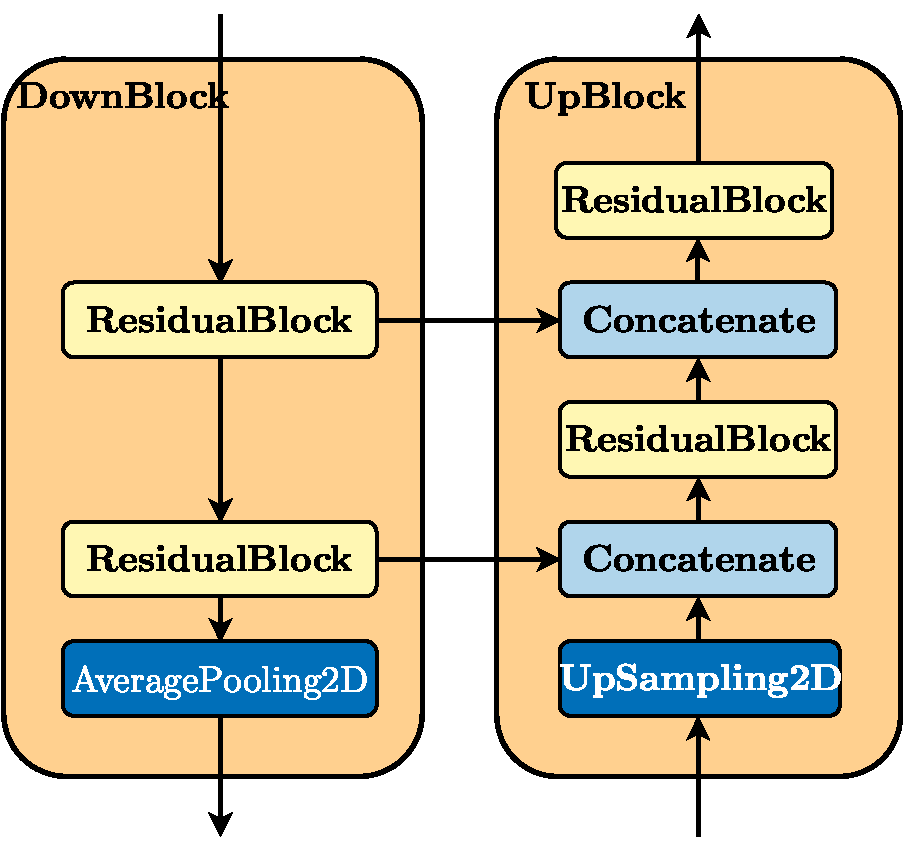
\includegraphics[keepaspectratio, scale=0.5]{UNET3.pdf}
    \caption{Dettagli dei blocchi “\emph{DownBlock}” e “\emph{UpBlock}” della U-Net di Figura~\ref{fig:UNet}. Fonte~\cite{fosterGenerativeDeepLearning2023}.}
    \label{fig:UNet_details}
\end{figure}